%growth rates not sig changed 
%v shear from thin dust layers are overwhelmed by 
\section{Discussion}\label{discussion}

\subsection{Generalization to locally polytropic disks}
We can extend the dusty/adiabatic gas correspondence to 
other fixed equations of state. As an example, consider the locally
polytropic disk 
\begin{align}
  P = K(r,z)\rhog^{\Gamma}, 
\end{align}
where $K$ is a prescribed function and $\Gamma$ is the constant
adiabatic index. Then eliminating $\tepsilon$ from the dust equation
\ref{dusteq} gives 
\begin{align}\label{poly_energy}
  \frac{D P}{D t} &= - \Gamma P\nabla\cdot\bm{v}  + P \bm{v}\cdot\nabla
  \ln{K} + \mathcal{C},\\
  \mathcal{C}& = \frac{\Gamma P}{\rhog}\nabla\cdot\left(\tepsilon\tstop\nabla
  P\right).
\end{align}
Thus the dusty gas behaves like a pure gas with adiabatic index
$\Gamma$. The entropy is given by 
\begin{align}
  s = \ln{\left[K^\frac{1}{\Gamma}(r,z)\left(1 - \tepsilon\right)\right]}.  
\end{align}
The results of \S\ref{iso_perfect}---\ref{dust_work} remain valid for the strictly 
polytropic disk with $K=$constant, while one can set $c_s^2\to K$ in
\S\ref{dusty_vsi_int}. 
%When $K$ is constant, the corresponding Solberg-Hoiland criteria for
%axisymmetric stability may be obtained from that in standard adiabatic 
%hydrodynamics \citep[e.g.][]{tassoul78} by
%using this definition of entropy in
%Eqs. \ref{dusty_solberg1}---\ref{dusty_solberg2}. 

\subsection{Implications for numerical simulations}
The dusty/adiabatic gas equivalence means that pure
gas dynamics codes can be applied to simulate locally
isothermal/polytropic dusty gas with minimal modification. In fact, no
modification is needed  
for strictly isothermal or polytropic gas perfectly-coupled to dust:  
the standard adiabatic energy equation substitutes for the dust continuity
equation. When $c_s$ or $K$ is not constant and/or $\tstop\neq0$ one
should add corresponding source terms in energy equation. 
This source term associated with dust-gas drag, $\mathcal{C}$, is 
analogous to radiative diffusion \citep{price15}, which is also
standard in many hydrodynamics codes.      

\subsection{Dusty analogs of other gaseous instabilities}  

%gi
%rwi 

\subsubsection{Gravitational instability} %vertical structure 
The addition of dust enhances gravitational
instability (GI). This is because dust particles contribute to the
total disk mass but not thermal pressure, which effectively lowers the
disk temperature \citep[][]{thompson88,shi13}. For typical dust-loading 
$\epsilon, Z\ll1$, this effect is unimportant. However, if $\epsilon$ is
large (e.g. due to dust settling) then the effective temperature may 
be lowered to enable instability. 

As noted in \S\ref{loc_iso_eos}, dust settling causes the effective
temperature to \emph{increase} away from the midplane. This contrasts
to previous studies of GI in vertically stratified disks
\citep[e.g.][]{mamat10, kim12,lin14c} where the temperature decreases
from the midplane. While we expect only the total surface density and
characteristic temperatures are relevant to stability  
\citep{toomre64}, having a non-trivial vertical temperature
structure, induced by dust, may modify the vertical structure of 3D
waves and unstable modes. We will examine this linear problem in a following 
study.  



%see also
%\S\ref{loc_iso_eos}
%We thus expect the standard Toomre
%parameter to be modified to $Q = c_s\sqrt{1-\tepsilon}\Omega/\pi
%G\Sigma$. 

\subsubsection{Rossby wave instability}
The Rossby wave instability (RWI) is a non-axisymmetric, 2D shear
instability that operates in thin disks when it has radial structure
\citep{lovelace99,li00}. These studies consider adiabatic pure gas and 
show instability is possible if there is an extrema in the quantity
\begin{align}
 \eta = \frac{\kappa^2}{2\Omega\Sigma}\mathcal{S}^{2/\gamma},  
\end{align} 
where $\mathcal{S} = \Pi/\Sigma^\gamma$. Here, $\Sigma$ is the total
surface density and $\Pi$ is the vertically integrated pressure. 

From the dusty/adiabatic gas equivalence, we deduce the corresponding
condition for RWI in a (locally isothermal or polytroipc) dusty gas is
also given by extrema in $\eta$ with $\mathcal{S} = \exp{s}$ (and
$\tepsilon\to \Sigma_\mathrm{d}/\Sigma$). Since
the dusty entropy $s$ reflects the dust distribution, we expect that
RWI may also be triggered by extrema in  the dust-to-gas ratio. 


%gap edges. thin dust rings. 

\subsection{New dust-drag
  instabilities}\label{dust_as_thermo} 

As described in \S\ref{dust_work}, 
the physical cause of dust-drag instabilities is a phase lag between
the pressure and density response in a dusty gas\footnote{
In fact, we expect a phase difference between pressure and the total
density  whenever $\tstop\neq0$; not just $\tstop\OmK\ll 1$ as 
considered in this work. This is simply because of the finite
relaxation time required for dust to respond to gas, and vice versa. 
An effective energy equation in the form of Eq. \ref{eff_energy} can
still be obtained for general $\tstop$. The
heat flux $\bm{F}$ in the cooling function $\mathcal{C}$ is determined
through solution to the relative velocity $\Delta \bm{v} =
\bm{v}_\mathrm{d}-\bm{v}_\mathrm{g}$ \citep{youdin05a,laibe14}.  We
thus expect the `pressure-density lag' interpretation of dust-drag 
instabilities to be generally applicable.}. 
This may be used to re-interpret the streaming instability or to
understand other dusty instabilities. For example,
\cite{loren15,loren16} have recently discovered a new axisymmetric 
instability in their two-fluid numerical simulations of dusty
protoplanetary disks. They find it leads to the formation of
`toroidal vortices'. 

%give numerical example 
We have applied our one-fluid stability analysis to find unstable modes  
similar to that described by \cite{loren15}. We use the same
parameters reported by them as follows. 
%we set $p=q=0$, which eliminates VSI and minimizes streaming
%instabilities as there is no radial pressure gradient at the disk
%midplane.   
The total metalicity is $Z=0.01$ and the dust scale-height $H_\mathrm{d} =
0.4H_\mathrm{g}$, giving a maximum dust-to-gas ratio
$\mathrm{max}(\epsilon) = 0.025$. The midplane stopping time is 
$t_\mathrm{s0}=0.02\OmK^{-1}$. The disk parameters are $p=-1.5,\, q=-1$, and  
$\hgas=0.05$. We set $k = \pi/H_\mathrm{d}$.      

Fig. \ref{compare_eigenvals_ts0d02} shows the unstable modes found for
this setup. We find the usual VSI modes, here with $\omega> 3,\, s<
0.2$. However, we also find modes with $\omega<s$. One of these,
marked by the blue asterisk, has 
frequency 
\begin{align*}
\sigma = (0.3631\ii - 0.1251)\hgas\OmK. 
\end{align*}
This growth rate corresponds to $8.8$ orbits, comparable to the $12$
orbits reported by \citeauthor{loren15}. We visualize this mode in
Fig. \ref{result2d_loren}. We find this mode 
persists when $q=0$, so it is not the VSI. 
Using Eq. \ref{streaming_dispersion} with the above parameters,  
we also estimate a much smaller growth 
rate for the streaming instability of 
$O(10^{-3}\hgas\OmK)$, We thus also rule out
SI, as did \citeauthor{loren15}. However, the mode disappears with
$\tstop=0$, so it is associated with finite dust-gas drag. 

\begin{figure}
  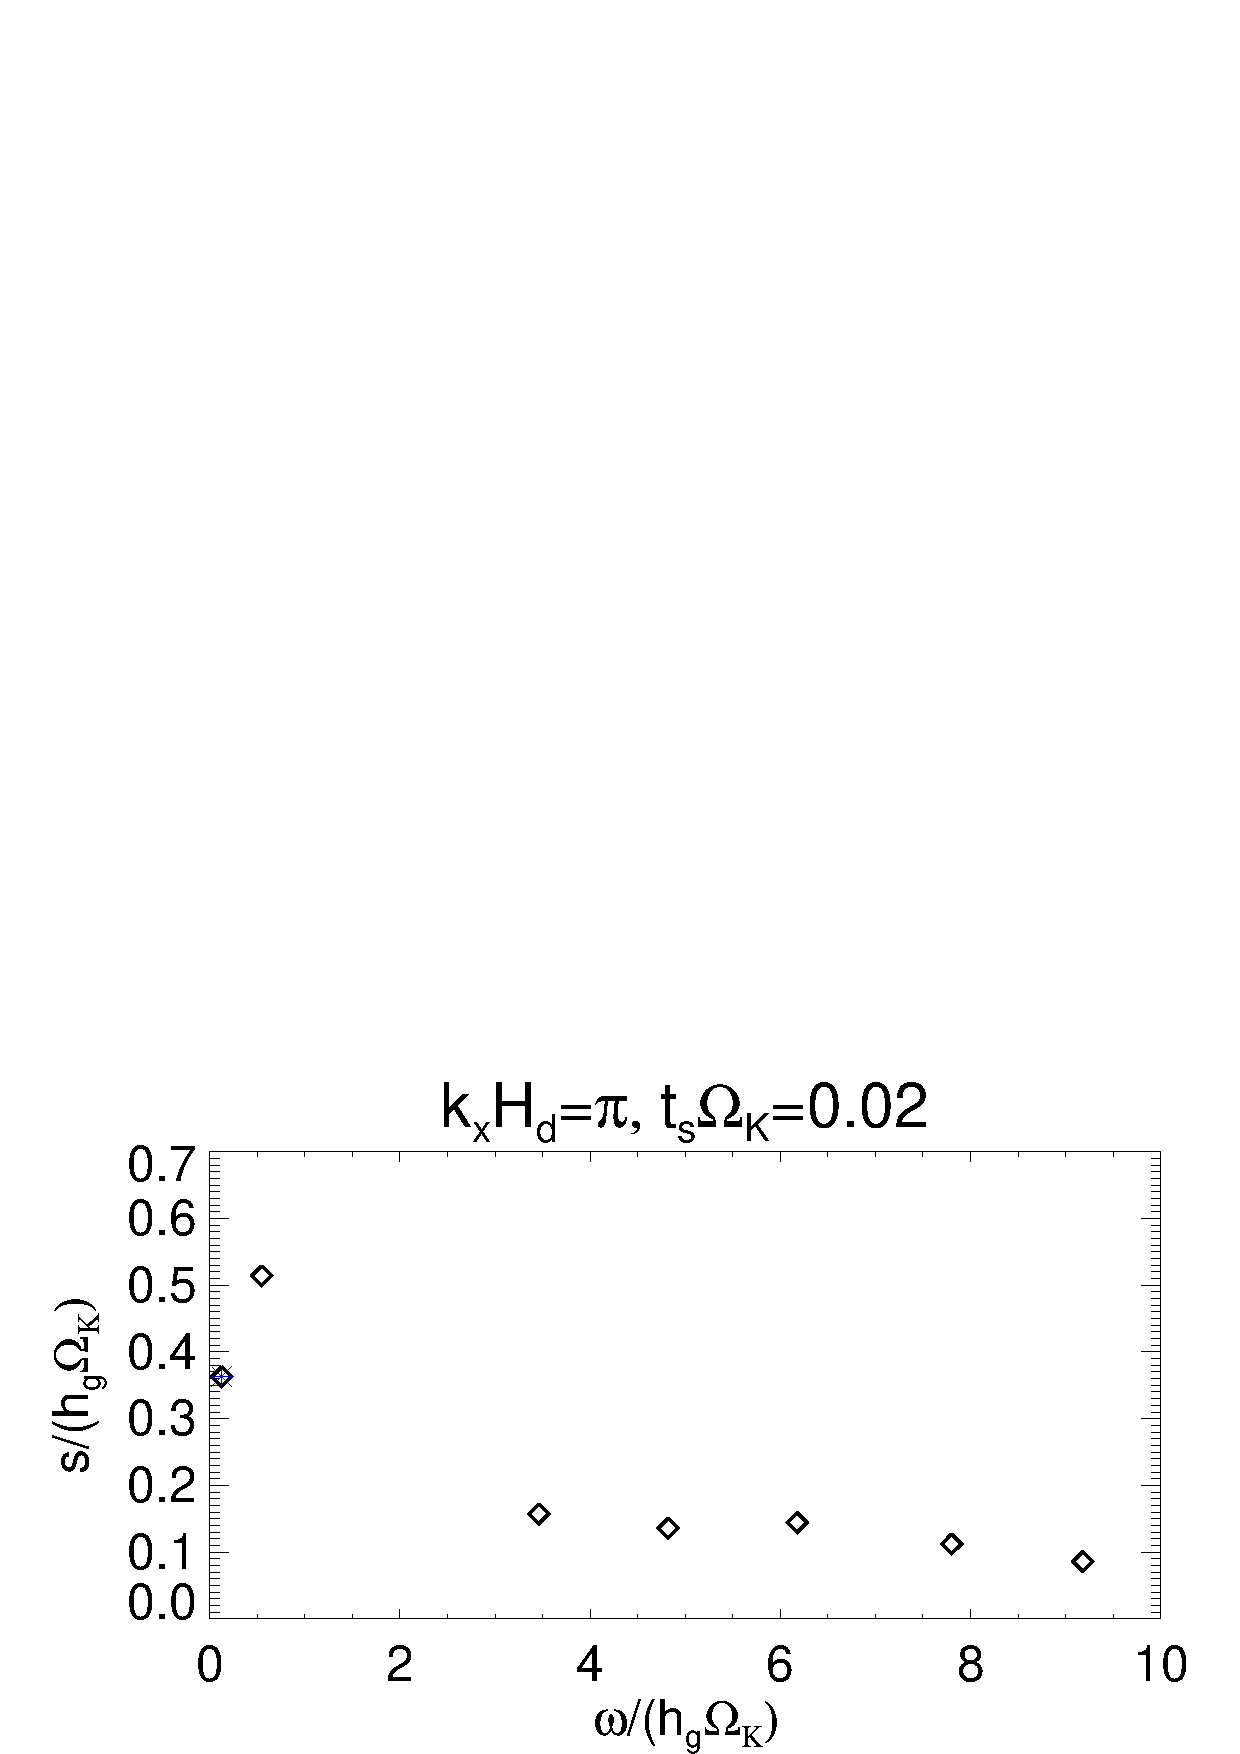
\includegraphics[width=\linewidth]{figures/compare_eigenvals_ts0d02}
  \caption{Unstable modes in a locally isothermal, dusty disk
    with stopping time  
    $\tstop=0.02\OmK^{-1}$. Modes with $\omega>3$ are due to
    VSI. The mode marked by the blue asterisk, visualized in
    Fig. \protect\ref{result2d_loren}
    , is associated with finite dust-gas
    drag. 
  }\label{compare_eigenvals_ts0d02}
\end{figure}


\begin{figure}
  \includegraphics[width=\linewidth]{figures/result2d_loren.ps}
  \caption{Visualization of the mode marked by the blue asterisk in
    Fig. \protect\ref{compare_eigenvals_ts0d02}. 
    This is a possible eigenmode of the dusty instability discovered by  
    \cite{loren15} in their numerical simulations. The instability growth timescale and 
    radial spacing of the `toroidal vortices' are similar to that 
    reported by \citeauthor{loren15}. This instability is driven by
    dust-gas drag. The color scale shows the 
    perturbed  
    dust-to-gas ratio, $\delta\epsilon$; and the arrows show
    $\sqrt{\rho}\left(\dd v_x, \dd v_z\right)$. 
  }\label{result2d_loren}
\end{figure}





This preliminary calculation only serves to highlight the possibility
of new axisymmetric dust-drag instabilities in stratified disks. One 
issue is that the base state for the above calculation is not a true
equilibrium (although \citeauthor {loren15} find the dust settling
time is longer than the instability growth time). We will study
this instability in more detail with a proper basic
state in a follow up work.  

\section{Summary}\label{summary}
In this paper we highlight the similarity between an isothermal 
dusty gas and an adiabatic, pure gas. The correspondence arises
because drag forces reduce the relative velocity between gas and
dust. In the limit of perfect dust-gas coupling, $\tstop \to 0$,  
 dust is entrained in 
the gas, and $\rhod/\rhog$ is conserved following the dusty flow. 
This is analogous to entropy being conserved following a adiabatic,
pure gas. 

For $\tstop\neq 0$, the dust content of a
fluid parcel of the dusty mixture no longer conserved. The parcel is
is allowed to exchange dust particles with neighboring parcels owing
to finite dust-gas friction. This is analogous to heat exchange between a 
pure gas parcel and its surroundings. %Thus, finite dust-gas friction
%may be interepreted as an energy source for the dusty
%gas.   

We explicitly show that for a locally isothermal, dusty gas that the
evolutionary equation of  $\rhod/\rhog$ may be replaced by an 
effective energy equation. We find the 
natural definition of the entropy of the dusty gas is 
\begin{align*}
  s  = \ln{\left(\frac{c_s^2\rhog}{\rhog+\rhod}\right)}.  
\end{align*}
%This allows us to define the buoyancy frequency of an isothermal 
%dusty gas. 
In our framework, finite dust-gas friction appears as an energy
source term.  This analogy with standard adiabatic
hydrodynamics allow us to obtain dusty analogs of gaseous
instabilities, and provide thermodynamical interpretations of  
dust-drag instabilities. 

%
In this first study, we apply this equivalence principle to study the
axisymmetric stability of isothermal, protoplanetary disks
perfectly coupled to dust ($\tstop=0$). This is so that we may 
compute exact, steady equilibria for analyses. Furthermore, 
in this limit the dusty problem is \emph{identical} to adiabatic, pure
gas dynamics. 

We obtain the Solberg-Hoiland criteria to assess 
axisymmetric stability when the equation of state is strictly
isothermal. We show that {\bf the vertical shear associated with thin dust
 layers, however large it is, cannot lead to axisymmetric
  instabilities} \citep[cf. \emph{non-axisymmetric} Kelvin-Helmholtz instabilities
  in dusty disks, ][]{lee10}. We show that
sharp edges in the dust-to-gas ratio cannot persist in protoplanetary
disks, as these imply a sharp entropy gradient and may thus destablize
the disk. 

%does not preclude non-axisymmetric instabilities. but if there is a
%global radial temp gradient, then vertical shear arising from
%it will always be comparable to dust-settling. but there is vsi with
%global rad temp grad 

For locally isothermal disks $c^2_s=c_s^2(r)$ we generalize the vertical
shear instability (VSI) to include dust. We find that dust-loading
generally has a stabilizing effect. In our disk models
dust-loading does not affect VSI growth rates significantly, but
meridional motions may be suppressed at heights where dust-induced
vertical buoyancy dominates over vertical shear, consistent with our
previous study \citep{lin15}.  

%These results are readily
%understood by comparing the vertical shear rate with the buoyancy of
%an isothermal, dusty gas which we have correctly identified. 

We also discuss future applications of our thermodynamic framework to 
study dusty protoplanetary disks. In particular, we emphasize  that the 
physical origin for any instability associated with strong dust-gas
drag is a phase lag between the pressure and total density evolution
of fluid elements. This leads to growing oscillations as positive work
is done, provided by dust-gas drag, which is equivalent to a `heat'
source. %We demonstrate a potentially new dust-drag instability in
%stratified disks that may explain 
 
%We also applied
%our framework to find unstable modes in dusty, stratified disks
%similar to that reported recently by \cite{loren15}. 
